% !TeX spellcheck = en_US
\section{Experiment properties}\label{section:properties}

In this chapter we will describe experiment configuration. To edit experiment configuration, you have to double click on .properties file in workspace tree.\\

Four windows are used to configure experiment:
\begin{itemize}
	\item \textbf{Properties form} - this is tab which opens after double click on properties file. It allows to edit experiment configuration.
	\item \textbf{Default properties form} - it is special case of properties form, where default properties for all experiments all configured.
	\item \textbf{Ranking dialog} - this modal dialog supports user friendly object ranking edition.
	\item \textbf{Pairs dialog} - this modal dialog supports user friendly comparison pairs edition
\end{itemize}

All windows are described in sections below.

\subsection{Properties form}\label{sub:properties-form}

With default user settings, properties form will be opened with hidden sections of properties. This sections can be expanded by clicking on them. You can change this settings in User settings dialog. See \hyperref[section:user-settings]{User settings section}.

On top of the form, there is learning and test data table path. Learning data file is required field. If you hover on field with default user settings, tooltip with help will be displayed. You should also configure ranking or pairs before running experiment.

\begin{figure*}[!ht] 
	\centering
	\makebox[\textwidth]{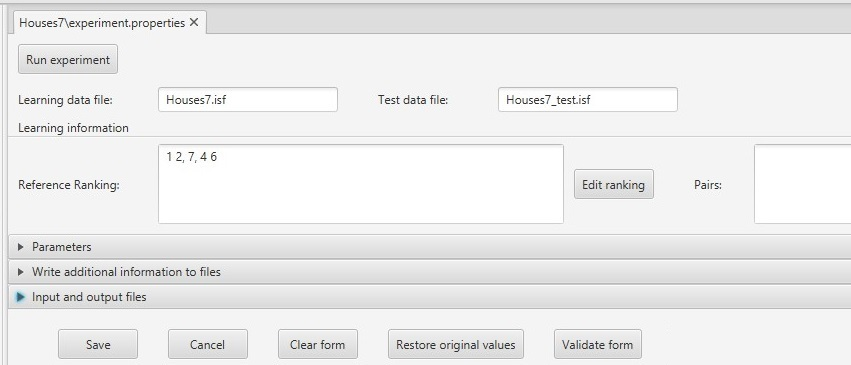
\includegraphics[width=.75\paperwidth]{properties}}
	\caption{Properties form with default settings}
\end{figure*}

On bottom of the screen following actions can be performed:
\begin{itemize}
	\item \textbf{Clear form} - clears all fields.
	\item \textbf{Restore original values} - restores values for all fields, as they were loaded from file again.
	\item \textbf{Validate form} - performs validation on form for all fields, including default ones. When running experiment, empty values from properties are replaced with default ones. It can discover issues with configuration, when values from form and default properties are not correctly set. If you find such issue, you should change settings in your experiment or in default properties.
\end{itemize}

Below, we describe meaning of all parameters.
\begin{itemize}
	\item \textbf{Learning data file} - absolute or relative path to learning isf file. Directories must be separated by $\backslash$ character.
	\item \textbf{Test data file} - absolute or relative path to test isf file. Directories must be separated by $\backslash$ character. If not configured, it is assumed, that learning file is also test file.
	\item \textbf{Reference ranking} - initial ranking of objects in experiment.
	\item \textbf{Pairs} - pairs of object in outranking $S$ or non-outranking $S^{c}$ relation.
	\item \textbf{Type of family criteria} - can be consistent or any.
	\item \textbf{Type of rules} - can be certain of possible.
	\item \textbf{Considered set of rules} - if exhaustive, virtual exhaustive set of rules will be considered, if minimal, explicit minimal set of rules induced by VC-DomLEM algorithm will be considered.
	\item \textbf{Consistency measure} - measure used to calculate lower approximations of $S$ and $S^{c}$ relations.
	\item \textbf{Consistency measure threshold} - floating point number from [0,1] for epsilon, epsilon* and rough membership, or greater or equal than 0 for epsilon'.
	\item \textbf{Ranking procedure} - method used for calculating ranking from preference graph.
	\item \textbf{Dominance} - dominance relation used to calculate approximations of $S$ and $S^{c}$ relations in PCT.
	\item \textbf{Dominance for pairs of ordinal values} - indicator of the considered definition of dominance pairs of ordinal values in PCT.
	\item \textbf{Satisfaction degrees in preference graph} - weights in the preference graph. Can be fuzzy (from [0,1]) or crisp (0 or 1). Fuzzy satisfaction degree cannot be used with DRSA with exhaustive set of possible rules and rough membership.
	\item \textbf{Fuzzy satisfaction degree calculation method} - method for calculating fuzzy satisfaction degree in preference graph. Can be maximum of credibility over covering rules (max credibility) or maximum product of credibility and coverage factor over covering rules.
	\item \textbf{Negative examples treatment for VCDRSA} - sets strategy for covering negative examples by rules in VC-DRSA.
	\item \textbf{Rule conditions selection method in VCDomLEM} - strategy of rule conditions selection, either base (it can employ only elementary conditions built using evaluations of a single pair of objects) or mix (denotes that each rule can employ elementary conditions built using evaluations of different pairs of objects).
	\item \textbf{Optimize rule consistency in VCDomLEMWrt} - set of pairs of objects with respect to which value of rule consistency measure optimized in VC-DomLEM algorithm is calculated. Can be lower (or upper) approximation of the preference relation for which a certain (or possible, respectively) rule is generated or entire preference relation (for certain rules only) – either approximation or set.
	\item \textbf{Allow empty rules in VCDomLEM} - if true, rules with empty condition part can be generated if they have good consistency.
	\item \textbf{Use edge regions in VCDomLEM} - if true, only pairs of objects from EDGE region will be used to create rules condition.
	\item \textbf{Write domination information} - if true, sections [P-dominating sets] and [P-dominated sets] will be saved to .apx file.
	\item \textbf{Write rule statistics} - if true, rule statistics will be saved in .rule file.
	\item \textbf{Write learning positive examples} - if true, learning positive examples will be written to .rules file.
	\item \textbf{Precision} - denotes precision of floating point numbers when saving files. -1 disables rounding.
	\item \textbf{PCT file} - absolute or relative path on which isf file for Partial Pairwise Comparison Table will be saved. Directories must be separated by $\backslash$ character. If not given, name of the file will be set using learning data file name.
	\item \textbf{PCT Apx file} - absolute or relative path to .apx file, where approximations from PCT table will be saved. Directories must be separated by $\backslash$ character. If not given, name of the file will be set using learning data file name.
	\item \textbf{PCT rules file} - absolute or relative path on which rules will be saved. Directories must be separated by $\backslash$ character. If not given, name of the file will be set using learning data file name.
	\item \textbf{Preference graph file} - absolute or relative path on which graph will be saved. Directories must be separated by $\backslash$ character. If not given, name of the file will be set using test data file name.
	\item \textbf{Ranking file} - absolute or relative path on which ranking file will be saved. Directories must be separated by $\backslash$ character. If not given, name of the file will be set using test data file name.
\end{itemize}

\subsection{Default properties}\label{sub:properties-default}

When performing experiment, all properties must be set. So if user leave empty fields, they must be replaced with some default values. RUDE application have configurable default properties, which should be located in main workspace directory with file name: default.properties. You can edit this file freely, but it is recommended to fill all fields from parameters and write additional information sections.

\begin{figure*}[!ht] 
	\centering
	\makebox[\textwidth]{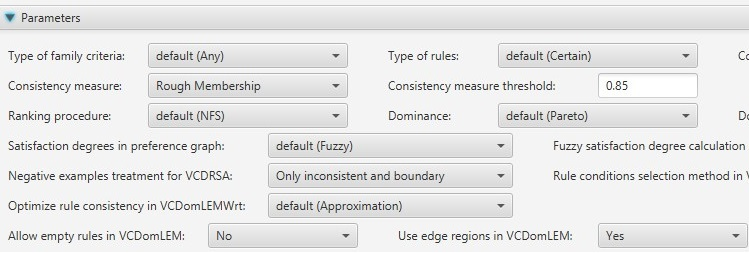
\includegraphics[width=.75\paperwidth]{properties-expanded}}
	\caption{Properties with default values set from default.properties file}
\end{figure*}

Default properties are loaded on each properties form. They are displayed to user in form: default (default value) for ComboBox fields, and as gray placeholder in other fields if they are empty. If you configure field in own experiment, value from your configuration will replace default one when performing experiment. All properties which are used in experiment are displayed in logs before experiment run.


\subsection{Ranking configuration}\label{sub:properties-ranking}

Ranking field represents initial ranking of objects in experiment. It can be edited by clicking on ''Edit ranking'' button.

Ranking can be configured manually in big text field, but it is not recommended and disabled by default. See \hyperref[section:user-settings]{User settings section}. Objects on left list are sorted by object ID.

\begin{figure*}[!ht] 
	\centering
	\makebox[\textwidth]{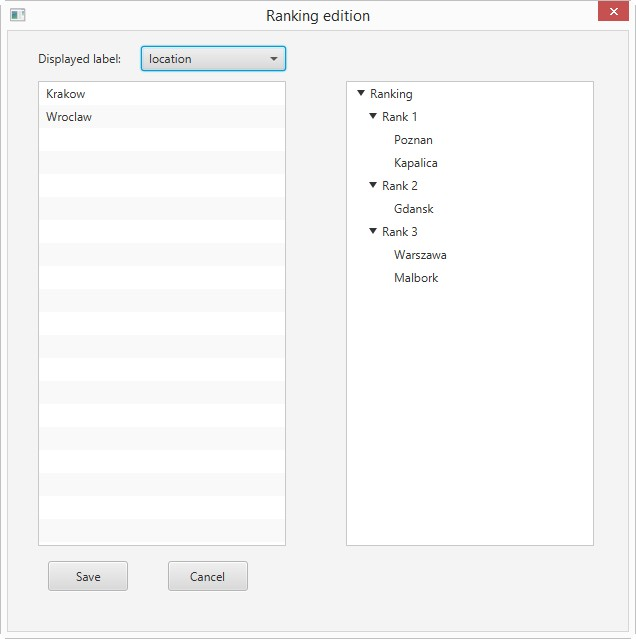
\includegraphics[width=.6\paperwidth]{properties-ranking}}
	\caption{Ranking edition modal dialog}
\end{figure*}

By default, objects ID (number of object) is displayed. If you created description attribute, it can be used as label for objects. You can change this in ''Displayed label'' field.

You can drag and drop objects from left list to right tree. If you place object on empty cell, new rank position will be created automatically. If you drag object to rank or element in rank, dragged object will be added to existing rank.

On right tree, you can perform two actions, which can be also invoked on selected item by context menu or keyboard shortcut:
\begin{itemize}
	\item \textbf{Remove selected (Delete)} - removes selected object from ranking. Removed object will return to list on the left. If rank was selected, all objects from rank will be removed to.
	\item \textbf{Add Rank below (A)} - adds new rank position below selected position.
\end{itemize}


\subsection{Pairs configuration}\label{sub:properties-pairs}

Pairs field represents comparison pairs of object in Pairwise Comparison Table. They can be edited by clicking on ''Edit pairs'' button.

Pairs can be configured manually in big text field, but it is not recommended and disabled by default. See \hyperref[section:user-settings]{User settings section}.

\begin{figure*}[!ht] 
	\centering
	\makebox[\textwidth]{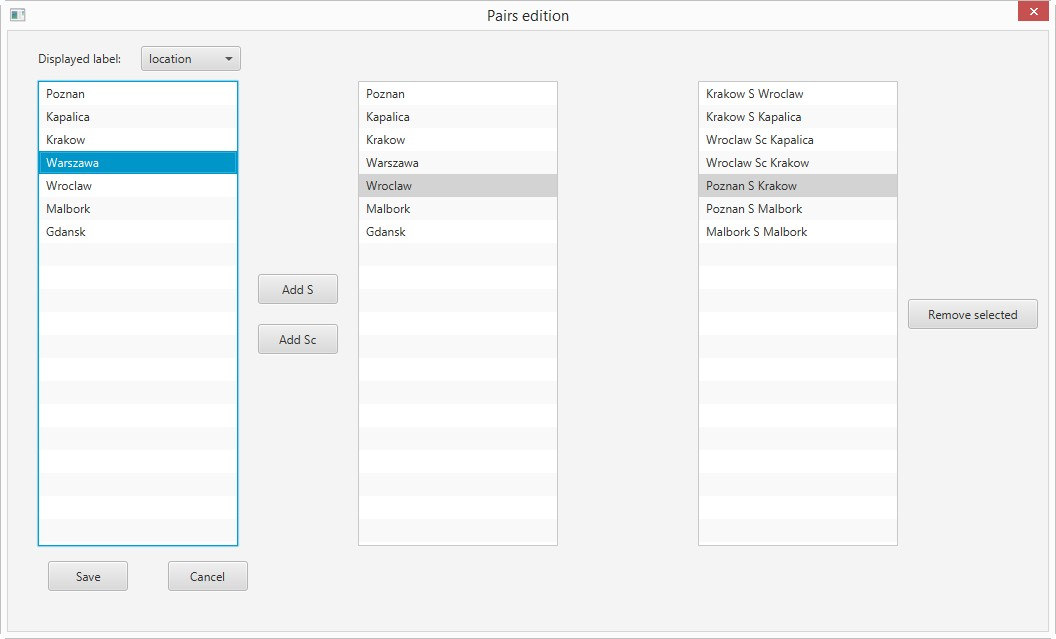
\includegraphics[width=.8\paperwidth]{properties-pairs}}
	\caption{Pairs edition modal dialog}
\end{figure*}

By default, objects ID (number of object) is displayed. If you created description attribute, it can be used as label for objects. You can change this in ''Displayed label'' field. 

First and second list contains all objects from experiment. Third list contains compared pairs of these objects with relation $S$ (outranking) or $S^{c}$ (non-outranking).

Three actions are available for this screen. Each can be invoked by pressing button, choosing option from context menu or by keyboard shortcut. First two actions are for first two lists, third is for pairs lists:
\begin{itemize}
	\item \textbf{Add S (S)} - adds selected pair of objects from first and second list to pairs lists. Objects are added in outranking relation.
	\item \textbf{Add Sc (C))} - adds selected pair of objects from first and second list to pairs lists. Objects are added in non-outranking relation.
	\item \textbf{Remove selected (Delete)} - removes selected pair from third list.
\end{itemize}



\vfill\newpage